% =====================================================================
% COSC 3337 — Homework 3 — Applications and Big Data
% =====================================================================
\documentclass[11pt]{article}

\usepackage[margin=1in]{geometry}
\usepackage{amsmath,amssymb}
\usepackage{booktabs}
\usepackage{enumitem}
\usepackage{fancyhdr}
\usepackage{xcolor}
\usepackage{textcomp}
\usepackage{listings}
\usepackage[most]{tcolorbox}
\usepackage{array}
\usepackage{tabularx}
\usepackage{tikz}
\usepackage{needspace}
\usetikzlibrary{positioning,arrows.meta}
\usepackage[hidelinks]{hyperref}

% ---- edit these ------------------------------------------------------
\newcommand{\hwnum}{3}
\newcommand{\released}{October 19, 2026}
\newcommand{\due}{November 1, 2026, 11:59 pm}
% ---------------------------------------------------------------------

\definecolor{boxred}{HTML}{C9605A}
\definecolor{boxredbg}{HTML}{FBF3F2}
\definecolor{boxblue}{HTML}{4A6F96}
\definecolor{boxbluebg}{HTML}{F2F6FA}
\definecolor{codegray}{HTML}{6B6B6B}

\newtcolorbox{warnbox}[1]{enhanced, breakable, colback=boxredbg, colframe=boxred,
  fonttitle=\bfseries\small, title={#1}, boxrule=0.6pt, arc=1pt,
  left=6pt, right=6pt, top=4pt, bottom=4pt}
\newtcolorbox{notebox}[1]{enhanced, breakable, colback=boxbluebg, colframe=boxblue,
  fonttitle=\bfseries\small, title={#1}, boxrule=0.6pt, arc=1pt,
  left=6pt, right=6pt, top=4pt, bottom=4pt}

\lstset{
  basicstyle=\ttfamily\small,
  columns=fullflexible,
  keepspaces=true,
  upquote=true,
  showstringspaces=false,
  frame=leftline,
  framerule=0.8pt,
  rulecolor=\color{codegray},
  xleftmargin=1.2em,
  framexleftmargin=0.6em,
  aboveskip=6pt,
  belowskip=6pt,
  commentstyle=\color{codegray},
  breaklines=true,
}
\lstdefinestyle{py}{language=Python}
\lstdefinestyle{sql}{language=SQL, morekeywords={LIMIT,COALESCE}}
\newcommand{\code}[1]{\texttt{#1}}
\newcommand{\pts}[1]{\hfill\textit{(#1 points)}}
\newcommand{\pt}[1]{\textit{(#1~pt\ifnum#1>1 s\fi)}}

\pagestyle{fancy}
\fancyhf{}
\lhead{\small COSC 3337 --- Homework \hwnum}
\rhead{\small Page \thepage}
\renewcommand{\headrulewidth}{0.4pt}

\setlength{\parindent}{0pt}
\setlength{\parskip}{6pt}
\setlength{\emergencystretch}{3em}
\setlist{itemsep=2pt, topsep=4pt}

\begin{document}

% =====================================================================
\begin{center}
  {\LARGE\bfseries Homework \hwnum: Applications and Big Data}\\[4pt]
  {\large COSC 3337 --- Databases --- Fall 2026}\\[6pt]
  \begin{tabular}{@{}ll@{}}
    \textbf{Released} & \released \\
    \textbf{Due}      & \due \\
    \textbf{Total}    & 100 points, plus 5 bonus
  \end{tabular}
\end{center}
\vspace{2pt}\hrule\vspace{10pt}

\section*{Before you start}

Databases often sit behind applications: a website or an app takes what a user clicks or types, turns
it into queries, and turns the results into a page. This homework is about that
layer, and about what changes when the data gets too big for one machine.

Everything uses a new database, \code{soundwave\_app}: the Soundwave catalog you
know from HW~1 (\code{artist}, \code{album}, \code{track}) plus the tables a
streaming application needs on top of it.

\begin{center}
\begin{tabular}{@{}l l@{}}
\toprule
\textbf{Table} & \textbf{Columns} (primary key underlined)\\
\midrule
\code{artist} & \underline{\code{artist\_id}}, \code{name}, \code{country}, \code{formed\_year}\\
\code{album}  & \underline{\code{album\_id}}, \code{title}, \code{artist\_id}, \code{release\_year}, \code{genre}\\
\code{track}  & \underline{\code{track\_id}}, \code{album\_id}, \code{title}, \code{duration\_sec}\\
\midrule
\code{listener}       & \underline{\code{listener\_id}}, \code{username}, \code{email}, \code{country}, \code{joined\_date}\\
\code{playlist}       & \underline{\code{playlist\_id}}, \code{listener\_id}, \code{name}, \code{created\_date}\\
\code{playlist\_track}& \underline{\code{playlist\_id}, \code{track\_id}}, \code{position}\\
\code{play}           & \underline{\code{play\_id}}, \code{listener\_id}, \code{track\_id}, \code{played\_at}\\
\bottomrule
\end{tabular}
\end{center}

A \code{play} row is written every time a listener plays a track.
\code{playlist\_id} and \code{play\_id} are \code{AUTO\_INCREMENT}.

\textbf{Part 1} is written (50 points). \textbf{Part 2} is code (50 points).

\textbf{What to submit:} one zip file containing exactly:
\begin{enumerate}[nosep]
  \item \code{hw3.pdf} --- your answers to Part 1.
  \item \code{app\_queries.py} --- your answers to Questions 2.1 and 2.2.
  \item \code{mapreduce\_jobs.py} --- your answers to Question 2.3.
\end{enumerate}
Do not rename the two \code{.py} files. The autograder looks for them by name.

\textbf{Typesetting bonus (5 points).}
\begin{itemize}
  \item \textbf{By hand.} You may hand-write Part 1. Submit a PDF made with a
  scanning app, not a photograph, with every question clearly labeled.
  \item \textbf{With \LaTeX\ (5 bonus points).} If you typeset Part 1 in \LaTeX,
  you earn 5 bonus points. A template, \code{hw3\_template.tex}, is in the
  \code{HW3} folder. Submit the compiled PDF, not the \code{.tex} file.
\end{itemize}

\textbf{Do Part 0 first, and early,} so we have time to fix any setup problems.

% =====================================================================
\section*{Part 0 --- Setup \hfill \textit{(0 points, required)}}

\subsection*{0.1 Get the starter code}

On your VM, go to your copy of the course repository, pull the new homework
from \code{upstream} (my repository, which you set up in HW~1, Part~0.4), and
load the new database:
\begin{lstlisting}
cd COSC3337-FA26-homeworks
git pull upstream main
cd HW3
bash setup_db.sh
\end{lstlisting}

A plain \code{git pull} pulls from \code{origin}, your own repository, which
does not have HW~3 yet. If \code{git pull upstream main} complains that
\code{upstream} does not exist, run \code{git remote -v}: you should see both
\code{origin} (your \code{cosc3337-work}) and \code{upstream} (mine). If
\code{upstream} is missing, add it and pull again:
\begin{lstlisting}
git remote add upstream https://github.com/isabelcachola/COSC3337-FA26-homeworks.git
git pull upstream main
\end{lstlisting}

\code{setup\_db.sh} loads \code{soundwave\_app}, installs the two Python packages
the starter code needs (the MySQL connector and \code{pytest}), and checks that
Python can connect. Like HW~1's script, it is safe to run again at any time and
restores \code{soundwave\_app} to a clean state, so it is your repair command.
Unlike HW~1, your code \emph{writes} to this database.

\subsection*{0.2 Run the tests}

\begin{lstlisting}
python3 -m pytest tests/ -v
\end{lstlisting}

Every test should run and \emph{fail} with \code{NotImplementedError}. That
means your setup works: the tests can import your files and reach the database.
Any other error (cannot connect, module not found) is a setup problem. Re-run
\code{setup\_db.sh}, and if that does not fix it, email me or come to office hours.

\subsection*{0.3 Back up your work}

Commit and push to your private \code{cosc3337-work} repository every time you
stop working, as in HW~1. From inside \code{HW3}:
\begin{lstlisting}
git add app_queries.py mapreduce_jobs.py
git commit -m "<what you did this session>"
git push
\end{lstlisting}
Your VM has no backup.

% =====================================================================
\newpage
\section*{Part 1 --- Written \hfill \textit{(50 points)}}

% ---------------------------------------------------------------------
\subsection*{1.1 Application architecture \pts{8}}

Soundwave's web player is a \emph{three-tier} application:

\begin{center}
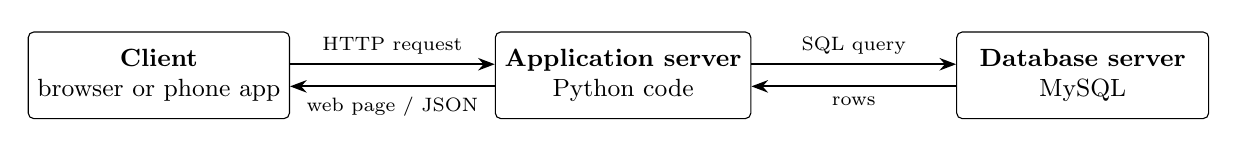
\begin{tikzpicture}[
  tier/.style={draw, rounded corners=2pt, minimum width=3.2cm, minimum height=1.1cm, align=center, font=\small},
  arr/.style={-{Stealth[length=6pt]}, thick}]
  \node[tier] (c) {\textbf{Client}\\ browser or phone app};
  \node[tier, right=2.6cm of c] (a) {\textbf{Application server}\\ Python code};
  \node[tier, right=2.6cm of a] (d) {\textbf{Database server}\\ MySQL};
  \draw[arr] ([yshift=4pt]c.east) -- node[above, font=\scriptsize]{HTTP request} ([yshift=4pt]a.west);
  \draw[arr] ([yshift=-4pt]a.west) -- node[below, font=\scriptsize]{web page / JSON} ([yshift=-4pt]c.east);
  \draw[arr] ([yshift=4pt]a.east) -- node[above, font=\scriptsize]{SQL query} ([yshift=4pt]d.west);
  \draw[arr] ([yshift=-4pt]d.west) -- node[below, font=\scriptsize]{rows} ([yshift=-4pt]a.east);
\end{tikzpicture}
\end{center}

The functions you write in Part 2 are the application server's code.

\begin{enumerate}[label=(\alph*)]
  \item \pt{3} A listener taps \emph{Play} on a track. In order, list what each
  of the three tiers does, from the tap to the music starting. Your list must
  include the SQL statement(s) the application server sends, written out in full
  for listener \code{L0042} and track \code{T00123}.

  \item \pt{3} Which tier should enforce the rule that a listener may only add
  tracks to \emph{their own} playlists? Justify your answer.

  \item \pt{2} Give two reasons the client should \emph{not} connect to MySQL
  directly.

\end{enumerate}

% ---------------------------------------------------------------------
\subsection*{1.2 User input and SQL \pts{12}}

Soundwave's login page runs this code. \code{name} is whatever the user types
into the \emph{Username} box.

\begin{lstlisting}[style=py]
name = input("Username: ")
query = "SELECT listener_id, username FROM listener WHERE username = '" + name + "'"
cursor.execute(query)
rows = cursor.fetchall()     # log in as the first row returned, if any
\end{lstlisting}

\begin{enumerate}[label=(\alph*)]
  \item \pt{3} The user types \code{neonfox42}. Write out the exact string that
  \code{query} holds, which is the SQL that MySQL receives.

  \item \pt{3} Now the user types:
\begin{lstlisting}
neonfox42' OR '1'='1
\end{lstlisting}
  Write out the exact SQL that MySQL receives. Which rows of \code{listener}
  does it return?

  \item \pt{3} Using \code{UNION}, write an input for the \emph{Username} box
  that makes this query return \emph{every listener's email address}. Then write
  out the SQL that MySQL receives.

  \item \pt{3} What you did in parts (b) and (c) is called \textbf{SQL
  injection}. The standard fix is a \textbf{parameterized query}: the SQL text
  contains a placeholder, \code{\%s}, and the value is passed to \code{execute}
  separately:
\begin{lstlisting}[style=py]
query = "SELECT listener_id, username FROM listener WHERE username = %s"
cursor.execute(query, (name,))
\end{lstlisting}
  What happens when your inputs from parts (b) and (c) are run through this
  version? Explain why it defeats both attacks.
\end{enumerate}

% ---------------------------------------------------------------------
\subsection*{1.3 Queries in a loop \pts{10}}

Soundwave's \emph{My Playlists} page shows each of a listener's playlists with
its number of tracks and total length. A first version of the code
(\code{get\_dashboard\_slow} in \code{app\_queries.py}) does this:

\begin{lstlisting}[style=py]
cur.execute("SELECT playlist_id, name FROM playlist WHERE listener_id = %s "
            "ORDER BY playlist_id", (listener_id,))
playlists = cur.fetchall()

for playlist_id, name in playlists:
    cur.execute("SELECT COUNT(*), SUM(t.duration_sec) "
                "FROM playlist_track pt JOIN track t ON pt.track_id = t.track_id "
                "WHERE pt.playlist_id = %s", (playlist_id,))
    ...
\end{lstlisting}

\begin{enumerate}[label=(\alph*)]
  \item \pt{2} How many queries does this send for a listener with $N$ playlists?

  \item \pt{6} Write \emph{one} SQL query that returns exactly what the code
  above returns for listener \code{L0042}:
  \code{(playlist\_id, name, num\_tracks, total\_duration\_sec)}, ordered by
  \code{playlist\_id}. 

  \item \pt{2} Many applications use an \emph{ORM} (object-relational mapper),
  a library that lets code treat rows as ordinary objects:
\begin{lstlisting}[style=py]
for pl in listener.playlists:
    print(pl.name, len(pl.tracks))
\end{lstlisting}
  How many queries might this code send for a listener with $N$ playlists?
  Compare it with \code{get\_dashboard\_slow}: which version makes the cost
  easier to see, and why?
\end{enumerate}

% ---------------------------------------------------------------------
\subsection*{1.4 Scaling out: sharding \pts{10}}

Soundwave's \code{play} table has grown to billions of rows, too many for one
server, so it is \emph{sharded}: split across 4 servers (``nodes''), each
holding some of the rows. Two schemes are proposed:

\begin{itemize}
  \item \textbf{Scheme H (hash):} a row goes to node
        $\mathit{hash}(\code{listener\_id}) \bmod 4$.
  \item \textbf{Scheme R (range):} a row goes to a node by \code{played\_at}:
        node 1 holds January--March 2026, node 2 April--June, node 3
        July--September, node 4 October--December.
\end{itemize}

\begin{enumerate}[label=(\alph*)]
  \item \pt{6} For each query below and each scheme, how many nodes must be
  contacted? Justify each of the six answers.
  \begin{enumerate}[label=\arabic*.]
    \item Listener \code{L0042}'s full play history (\emph{Recently played}).
    \item The number of plays of each track during March 2026.
    \item Inserting the row for a play that is happening right now.
  \end{enumerate}

  \item \pt{4} A \emph{hot spot} is a node that receives far more work than the
  others. Does either scheme create hot spots? Explain.

\end{enumerate}

% ---------------------------------------------------------------------
\subsection*{1.5 MapReduce by hand \pts{10}}

\emph{MapReduce} computes over data spread across many machines in three steps:
\begin{enumerate}[nosep]
  \item \textbf{Map:} a function you write is called on each input record, on
  whichever machine holds it, and emits zero or more \emph{(key, value)} pairs.
  \item \textbf{Shuffle:} the framework collects all pairs with the same key
  onto the same machine, producing \emph{key $\rightarrow$ [values]}.
  \item \textbf{Reduce:} a second function you write is called once per key, on
  that key's list of values, and emits the result for that key.
\end{enumerate}

\needspace{9\baselineskip}
Here are ten rows of the play log (with each track's genre already attached):

\begin{center}
\small
\begin{tabular}{@{}cccc@{\hspace{2.5em}}cccc@{}}
\toprule
\code{play\_id} & \code{listener} & \code{track} & \code{genre} &
\code{play\_id} & \code{listener} & \code{track} & \code{genre}\\
\midrule
1 & L01 & T05 & Folk  &  6 & L01 & T11 & Rock\\
2 & L02 & T11 & Rock  &  7 & L03 & T09 & Indie\\
3 & L01 & T07 & Folk  &  8 & L02 & T02 & Indie\\
4 & L03 & T02 & Indie &  9 & L01 & T05 & Folk\\
5 & L02 & T05 & Folk  & 10 & L03 & T13 & Rock\\
\bottomrule
\end{tabular}
\end{center}

The goal is the number of plays per genre.

\begin{enumerate}[label=(\alph*)]
  \item \pt{2} Write the \emph{(key, value)} pair the map function emits for
  each of the ten rows.
  \item \pt{2} Write the output of the shuffle.
  \item \pt{2} Write the output of each reduce call.
  \item \pt{2} Write the SQL query that computes the same thing from the
  \code{soundwave\_app} tables. Which part of your query corresponds to the
  shuffle?
  \item \pt{2} Suppose the play log is split across 100 machines. Describe how
  the work of each step is divided among them and what, if anything, has to move
  between machines. Why does this make MapReduce suitable for data too big for
  one database server?
\end{enumerate}

% =====================================================================
\newpage
\section*{Part 2 --- Code \hfill \textit{(50 points)}}

\subsection*{The files}

\begin{center}
\begin{tabularx}{\linewidth}{@{}l X l@{}}
\toprule
\textbf{File} & \textbf{What it is} & \textbf{You\ldots}\\
\midrule
\code{app\_queries.py}     & 2.1 and 2.2                                         & \textbf{edit and submit}\\
\code{mapreduce\_jobs.py}  & 2.3                                                & \textbf{edit and submit}\\
\code{db.py}               & \code{get\_connection()} and \code{QueryCounter}  & use, don't edit\\
\code{mapreduce\_driver.py}& \code{run\_mapreduce()} and \code{read\_plays()}  & use, don't edit\\
\code{data/plays.csv}      & the \code{play} table exported with \code{artist\_id} and \code{genre} & read\\
\code{tests/}              & the public tests                                  & run\\
\bottomrule
\end{tabularx}
\end{center}

Every function you write has a docstring that is its full specification: what
it receives, what it returns, in what order, and with examples. Read it before
you start the function. \textbf{Do not rename functions or change their
parameters}; the autograder calls them exactly as written.

\begin{notebox}{How grading works}
The autograder runs the public tests in \code{tests/} \emph{plus} hidden tests
for edge cases, on a \textbf{different copy of the data} (different listeners,
playlists and plays). Passing every public test means your functions have the
right shape. It does not guarantee full marks.
\end{notebox}

\subsection*{Python and MySQL}

\begin{lstlisting}[style=py]
from db import get_connection
conn = get_connection()                       # autocommit is OFF
cur = conn.cursor()
cur.execute("SELECT name, formed_year FROM artist "
            "WHERE country = %s AND formed_year > %s", ("Spain", 2010))
for name, year in cur.fetchall():             # a list of tuples
    print(name, year)
cur.close()
\end{lstlisting}

\begin{itemize}
  \item Every value from outside the program goes in through a \code{\%s}
  placeholder and the second argument of \code{execute}, which is always a
  tuple. Never put quotes around \code{\%s}: the connector handles quoting.
  To match part of a string, put the wildcards in the value:
  \lstinline|cur.execute("... LIKE %s", ("%" + text + "%",))|.
  \item \code{fetchall()} returns a list of tuples; \code{fetchone()} returns
  one tuple, or \code{None}.
  \item After an \code{INSERT} into a table with an \code{AUTO\_INCREMENT} key,
  \code{cur.lastrowid} holds the key MySQL just assigned.
\end{itemize}

\begin{notebox}{Commit and rollback}
With autocommit off, every change you make is \emph{provisional}. Your own
connection can see it, but no one else can, and it is not saved.
\begin{itemize}[nosep]
  \item \code{conn.commit()} makes every provisional change since the last
  commit permanent and visible to everyone.
  \item \code{conn.rollback()} throws every provisional change since the last
  commit away, as if it never happened.
\end{itemize}
This is how you make several statements \emph{all or nothing}: do them all,
then commit; if any one fails, roll back. When a statement violates a primary
key or foreign key, the connector raises \code{mysql.connector.IntegrityError},
which you can catch:
\begin{lstlisting}[style=py]
import mysql.connector
try:
    ...
except mysql.connector.IntegrityError:
    ...
\end{lstlisting}
\end{notebox}

\subsection*{2.1 Database-backed functions \pts{20}}

In \code{app\_queries.py}, write these three functions. Use parameterized
queries for every one.

\begin{itemize}
  \item \code{get\_top\_songs(conn, artist\_id, k)} --- an artist's \code{k}
  most-played tracks as \code{(track\_id, title, play\_count)}. Tracks that were
  never played still count, with 0.
  \item \code{create\_playlist(conn, listener\_id, name, track\_ids)} --- create
  a playlist and its tracks and return the new \code{playlist\_id}. On any bad input, raise \code{ValueError} and leave no rows behind.
  \item \code{search\_songs(conn, text)} --- every track whose title contains
  \code{text}, as \code{(track\_id, title, artist\_name)}. \code{text} is
  untrusted user input; implement your function with protections against SQL injection (see Question 1.2).
\end{itemize}

\begin{center}
\small
\begin{tabularx}{\linewidth}{@{}X r@{}}
\toprule
\textbf{What is tested} & \textbf{Points}\\
\midrule
\code{get\_top\_songs}: correct rows and order for several artists and values of \code{k} & 4\\
\code{get\_top\_songs}: ties, \code{k} larger than the catalog, never-played and unknown artists & 2\\
\code{create\_playlist}: valid input creates the rows, commits, returns the new id & 4\\
\code{create\_playlist}: bad input raises \code{ValueError} and \emph{no} rows remain & 4\\
\code{search\_songs}: correct matches, case-insensitive, including titles with apostrophes & 3\\
\code{search\_songs}: inputs like those in Question 1.2 return no extra rows and do not crash & 3\\
\bottomrule
\end{tabularx}
\end{center}

\subsection*{2.2 Speed up the dashboard \pts{10}}

\code{get\_dashboard\_slow} (Question 1.3) is provided and correct. Write
\code{get\_dashboard(conn, listener\_id)} so that it returns \emph{exactly} the
same thing for every listener, using \emph{at most 2 queries}, however many
playlists the listener has.

\code{db.QueryCounter} wraps a connection and counts the queries sent through
it. The autograder uses it to check you, so you can check yourself first:

\begin{lstlisting}[style=py]
from db import get_connection, QueryCounter
qc = QueryCounter(get_connection())
get_dashboard(qc, "L0001")
print(qc.count, qc.queries)
\end{lstlisting}

\begin{center}
\small
\begin{tabularx}{\linewidth}{@{}X r@{}}
\toprule
\textbf{What is tested} & \textbf{Points}\\
\midrule
Output identical to \code{get\_dashboard\_slow}, including listeners with no playlists and empty playlists & 5\\
At most 2 queries (\emph{only awarded if the output is also correct}) & 5\\
\bottomrule
\end{tabularx}
\end{center}

\subsection*{2.3 MapReduce in Python \pts{20}}

\code{mapreduce\_driver.py} contains a tiny single-machine MapReduce,
\code{run\_mapreduce(records, map\_fn, reduce\_fn)}. It calls \code{map\_fn} on
every record, does the shuffle, and calls \code{reduce\_fn} once per key,
exactly the three steps from Question 1.5. You write only the map and reduce functions,
in \code{mapreduce\_jobs.py}.

\begin{itemize}
  \item \textbf{Job 1, plays per genre.} \code{genre\_map} and
  \code{genre\_reduce}. This is Question 1.5 in code.
  \item \textbf{Job 2, each listener's most-played artist.} This needs
  \emph{two} MapReduce stages, because counting plays needs one grouping (by
  listener and artist) and picking the maximum needs another (by listener).
  Stage~1 is \code{count\_map}/\code{count\_reduce}; Stage~2 is
  \code{top\_map}/\code{top\_reduce}, and its input records are Stage~1's output
  pairs. \code{top\_artist\_job} chains them. Ties go to the smaller
  \code{artist\_id}.
\end{itemize}

The public tests check both jobs against the same question asked in SQL, so
when they pass, MapReduce and SQL agree.

\begin{warnbox}{Rules for Question 2.3 (checked by the autograder)}
\begin{itemize}[nosep]
  \item \code{mapreduce\_jobs.py} may not import \code{pandas}, \code{numpy},
  \code{sqlite3}, \code{mysql}, \code{pymysql} or \code{collections}.
  \item A mapper sees one record; a reducer sees one key and its values. Do not
  group values yourself; that is the shuffle's job.
\end{itemize}
\end{warnbox}

\begin{center}
\small
\begin{tabularx}{\linewidth}{@{}X r@{}}
\toprule
\textbf{What is tested} & \textbf{Points}\\
\midrule
\code{genre\_map} emits the right pair & 2\\
\code{genre\_reduce} returns the right pair & 2\\
Job 1 on the full play log equals the SQL \code{GROUP BY} answer & 4\\
Stage 1 of Job 2 (plays per listener and artist) is correct & 3\\
\code{top\_map} and \code{top\_reduce} are correct, including ties & 3\\
\code{top\_artist\_job} on the full play log equals the SQL answer & 4\\
No forbidden imports (\emph{only awarded if Job 1 is implemented}) & 2\\
\bottomrule
\end{tabularx}
\end{center}

\subsection*{Before you submit}

\begin{enumerate}[nosep]
  \item \code{python3 -m pytest tests/ -v} passes.
  \item You tested edge cases the public tests do not cover.
  \item Your zip contains \code{hw3.pdf}, \code{app\_queries.py} and
  \code{mapreduce\_jobs.py}, with those exact names.
\end{enumerate}

\end{document}
